\section{Vettori in $\mathbb{R}^3$}
Se vogliamo descrivere un punto nello spazio, è necessario definire cos'è lo spazio:

Prendiamo una terna destrorsa di assi cartesiani $\Rightarrow$ Descrivo $\mathbb{R}^3$.

\begin{center}
    \tdplotsetmaincoords{70}{110}

    \begin{tikzpicture}[tdplot_main_coords, scale=3]

        % Assi cartesiani
        \draw[->, thick] (0,0,0) -- (1.5,0,0) node[anchor=north east]{$x$};
        \draw[->, thick] (0,0,0) -- (0,1.5,0) node[anchor=north west]{$y$};
        \draw[->, thick] (0,0,0) -- (0,0,1.5) node[anchor=south]{$z$};

        % Coordinate del punto A
        \def\xa{1.2}
        \def\ya{0.8}
        \def\za{1.0}

        % Punto A
        \filldraw[ocra] (\xa,\ya,\za) circle (0.8pt)
            node[anchor=south west] {$A(\textcolor{red}{\xa},\textcolor{blue}{\ya},\textcolor{green!60!black}{\za})$};

        % Vettore r = OA
        \draw[->, very thick, purple] (0,0,0) -- (\xa,\ya,\za)
            node[midway, above left] {$\vec r$};

        % Proiezione su piano xy
        \draw[dashed] (\xa,\ya,\za) -- (\xa,\ya,0);
        \draw[dashed] (\xa,\ya,0) -- (\xa,0,0);
        \draw[dashed] (\xa,\ya,0) -- (0,\ya,0);

        % Componenti cartesiane colorate
        \draw[very thick, red] (0,0,0) -- (\xa,0,0)
            node[midway, below] {$\textcolor{red}{x_A}$};

        \draw[very thick, blue] (\xa,0,0) -- (\xa,\ya,0)
            node[midway, right] {$\textcolor{blue}{y_A}$};

        \draw[very thick, green!60!black] (\xa,\ya,0) -- (\xa,\ya,\za)
            node[midway, right] {$\textcolor{green!60!black}{z_A}$};

    \end{tikzpicture}
\end{center}

Considero un vettore $\vec r = (O-A)$, esso non è altro che una terna di valori ordinati $\vec r = (x_A, y_A, z_A)$.

Definisco il \textbf{modulo}, o lunghezza, di un vettore come: $\left | \vec v\right |=\sqrt{x^2 + y^2 +z^2} $

Se $\alpha \in \mathbb{R}$, posso definire $\vec u = \alpha \vec v$, e sarà un vettore che giace sulla stessa retta (ha la stessa direzione) di $\vec v$, verso come $sgn (\alpha)$ e modulo $\left | \vec u\right |=\left |\alpha \right |\left |\vec v\right |$.

Farà anche comodo definire un \textbf{Versore}, cioè un vettore con modulo unitario, che indicherò con $\hat u$.

\begin{example}
    Se volessi individuare $\hat v \parallel  \vec v$ è sufficiente fare: $\hat v = \frac{\vec v}{|\vec v|}$
\end{example}

Le operazioni elementari che si possono fare con i vettori sono:

\subsection{Prodotto scalare}
È una funzione che prende due vettori e restituisce uno scalare.

Presi due vettori $\vec u$ e $\vec v \in \mathbb{R}^3$, il prodotto scalare è definito come:
\begin{equation*}
    \left< \vec u, \vec v \right> = \vec u \cdot \vec v \in \mathbb{R}
\end{equation*}

Esso è una mappa con le seguenti proprietà:
\begin{itemize}
    \item \textbf{Simmetria}: $\left< \vec u, \vec v \right> = \left< \vec v, \vec u \right> $ con $\vec u, \vec v \in \mathbb{R}^3$
    \item \textbf{Linearità}: $\left< \alpha \vec u + \beta \vec w, \vec v \right> = \alpha \left< \vec u, \vec v \right> + \beta \left< \vec w, \vec v \right> $ con $\alpha, \beta \in \mathbb{R}$ e $\vec u, \vec v, \vec w \in \mathbb{R}^3$
\end{itemize}

La definizione standard ci dice che:
\begin{equation*}
    \left< \vec u, \vec v \right> = |\vec u||\vec v|\cos \theta
\end{equation*}
dove $\theta$ è l'angolo compreso tra i due vettori. (Non è importante quale dei due angoli si prenda, poiché il coseno è una funzione pari).

Se invece $\vec u = (u_x, u_y, u_z)$ e $\vec v = (v_x, v_y, v_z)$, allora: 
\begin{equation*}
    \left< \vec u, \vec v \right> = u_x v_x + u_y v_y + u_z v_z
\end{equation*}

\subsection{Prodotto vettoriale}
È sempre una mappa bilineare, ma restituisce un vettore invece di uno scalare.

\begin{minipage}
    {0.45\textwidth}
    \begin{equation*}
        \mathbb{R}^3 \times \mathbb{R}^3 \to \mathbb{R}^3
    \end{equation*}
    \begin{equation*}
        \vec u \wedge \vec v \mapsto \vec w
    \end{equation*}
\end{minipage}
\begin{minipage}
    {0.45\textwidth}
    \begin{center}
    \tdplotsetmaincoords{70}{120}
    \begin{tikzpicture}[tdplot_main_coords, scale=3]

        % Definizione vettori
        \def\ux{1}
        \def\uy{0.5}
        \def\uz{0.2}

        \def\vx{0.4}
        \def\vy{1}
        \def\vz{0.3}

        \pgfmathsetmacro{\wx}{\uy*\vz - \uz*\vy}
        \pgfmathsetmacro{\wy}{\uz*\vx - \ux*\vz}
        \pgfmathsetmacro{\wz}{\ux*\vy - \uy*\vx}

        % Piano generato da u e v
        \filldraw[blue!10, opacity=0.5]
            (0,0,0) -- (\ux,\uy,\uz) -- 
            ({\ux+\vx},{\uy+\vy},{\uz+\vz}) --
            (\vx,\vy,\vz) -- cycle;

        % Vettore u
        \draw[->, very thick, red]
            (0,0,0) -- (\ux,\uy,\uz)
            node[above left] {$\vec u$};

        % Vettore v
        \draw[->, very thick, green!60!black]
            (0,0,0) -- (\vx,\vy,\vz)
            node[above right] {$\vec v$};

        % Prodotto vettoriale
        \draw[->, very thick, blue]
            (0,0,0) -- (\wx,\wy,\wz)
            node[above] {$\vec w$};

    \end{tikzpicture}
    \end{center}
\end{minipage}

Possiamo ricavare le caratteristiche di $\vec w$:
\begin{itemize}
    \item $|\vec w| = |\vec u \wedge \vec v| = |\vec u||\vec v|\sin \theta$, dove $\theta$ è l'angolo compreso tra i due vettori.
    \item $\vec w$ è diretto cme la direzione $\perp$ al piano generato da $\vec u$ e $\vec v$.
    \item $\vec u$, $\vec v$ e $\vec w$ formano una terna destrorsa.
\end{itemize}

Le sue proprietà sono:
\begin{itemize}
    \item \textbf{Anticommutatività}: $\vec u \wedge \vec v = - \vec v \wedge \vec u$ con $\vec u, \vec v \in \mathbb{R}^3$
    \item \textbf{Linearità}: $\left( \alpha \vec u + \beta \vec w \right) \wedge \vec v = \alpha \left( \vec u \wedge \vec v \right) + \beta \left( \vec w \wedge \vec v \right)$ con $\alpha, \beta \in \mathbb{R}$ e $\vec u, \vec v, \vec w \in \mathbb{R}^3$
\end{itemize}

Geometricamente, il modulo di $\vec w$ rappresenta l'area del parallelogramma generato da $\vec u$ e $\vec v$.

\subsection{Terna euclidea}
Per fissare una terna euclidea non conviene definire tre vettori qualsiasi, ma è più comodo definire \textbf{tre versori ortonormali}.

Li chiamo $\hat i$, $\hat j$ e $\hat k$, rispettivamente paralleli agli assi $x$, $y$ e $z$.

\textbf{N.B.} Talvolta fa comodo fare distinzioni tra:
\begin{itemize}
    \item \textbf{Vettore libero} -- Fisso solo la direzione, ma non il punto di applicazione. Es. Velocità angolare.
    \item \textbf{Vettore Applicato} -- Fisso un punto di applicazione, oltre alla direzione. Es. Forza peso.
\end{itemize}

Il termine \textbf{ORTONORMALE} significa che i versori sono tra loro ortogonali:
\begin{equation*}
    \left< \hat i, \hat j \right> = \left< \hat j, \hat k \right> = \left< \hat k, \hat i \right> = 0
\end{equation*}
e sono normalizzati:
\begin{equation*}
    \left< \hat i, \hat i \right> = \left< \hat j, \hat j \right> = \left< \hat k, \hat k \right> = 1
\end{equation*}

Su tali versori è utile studiare il prodotto vettoriale:

\begin{minipage}
    {0.45\textwidth}
    \begin{equation*}
        \hat i \wedge \hat j = \hat k, \quad \hat j \wedge \hat k = \hat i, \quad \hat k \wedge \hat i = \hat j
    \end{equation*}
\end{minipage}
\begin{minipage}
    {0.45\textwidth}
    \begin{center}
    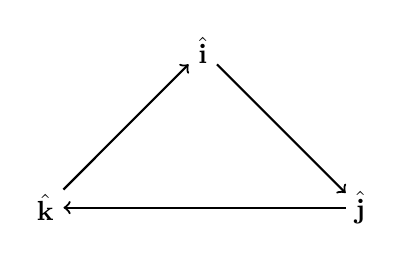
\begin{tikzpicture}[scale=2]

    % Posizione dei versori
    \node (i) at (0,1)   {$\hat{\mathbf i}$};
    \node (j) at (1,0)   {$\hat{\mathbf j}$};
    \node (k) at (-1,0)  {$\hat{\mathbf k}$};

    % Frecce cicliche
    \draw[->, thick] 
        (i) -- (j);

    \draw[->, thick] 
        (j) -- (k);

    \draw[->, thick] 
        (k) -- (i);

    \end{tikzpicture}
    \end{center}
\end{minipage}

Il vantaggio di definirie i versori è che ogni vettore $\vec v$ può essere scritto come combinazione lineare dei versori:
\begin{equation*}
    \vec v = \begin{pmatrix}
    v_x \\
    v_y \\
    v_z
    \end{pmatrix} = v_x \hat i + v_y \hat j + v_z \hat k
\end{equation*}

Data questa notazione, vediamo come posso ricavare le componenti di un vettore $\vec w = \vec u \wedge \vec v$:
\begin{align*}
    \vec u \wedge \vec v &= (u_x \hat i + u_y \hat j + u_z \hat k) \wedge (v_x \hat i + v_y \hat j + v_z \hat k) \\
    &= u_x v_x (\hat i \wedge \hat i) + u_x v_y (\hat i \wedge \hat j) + u_x v_z (\hat i \wedge \hat k) + u_y v_x (\hat j \wedge \hat i) + \\
    &+ u_y v_y (\hat j \wedge \hat j) + u_y v_z (\hat j \wedge \hat k) + u_z v_x (\hat k \wedge \hat i) + u_z v_y (\hat k \wedge \hat j) + u_z v_z (\hat k \wedge \hat k) \\
    &= (u_y v_z - u_z v_y) \hat i + (u_z v_x - u_x v_z) \hat j + (u_x v_y - u_y v_x) \hat k
\end{align*}

Un modo più compatto per ricordare questa formula è utilizzare il determinante (nonostante non sia un vero e proprio determinante, ma è solo una notazione mnemonica):
\begin{equation*}
    \vec u \wedge \vec v = \begin{vmatrix}
    \hat i & \hat j & \hat k \\
    u_x & u_y & u_z \\
    v_x & v_y & v_z
    \end{vmatrix}
\end{equation*}

\subsection{Momento di un vettore rispetto al polo}
Dato un punto $O$ detto "polo" e un vettore $\vec v$ applicato in un punto $P$, posso definire il momento di $\vec v$ rispetto ad $O$, come:

\begin{minipage}
    {0.45\textwidth}
    \begin{equation*}
        \vec M_O \doteq (P-O) \wedge \vec v
    \end{equation*}

    Dalla definizione di prodotto vettoriale, si deduce che $\vec{M_O}$ è un vetttore allineato con la normale al piano generato da $(P-O)$ e $\vec v$, e i tre vettori formano una terna destrorsa.
\end{minipage}
\begin{minipage}
    {0.45\textwidth}
    \begin{center}
    \begin{tikzpicture}[scale=1.5]

    % Assi
    \draw[->, thick] (-0.2,0) -- (3,0) node[right] {$x$};
    \draw[->, thick] (0,-0.2) -- (0,2.5) node[above] {$z$};

    % Punto O
    \coordinate (O) at (0.3,0.2);
    \filldraw[blue] (O) circle (1pt);
    \node[left] at (O) {$O$};

    % Punto P
    \coordinate (P) at (2,1.5);
    \node[right] at (P) {$P$};

    % Vettore u = P - O
    \draw[->, very thick, red] (O) -- (P)
    node[midway, above left] {$\mathbf{u} = (P-O)$};

    % Vettore v applicato in P
    \coordinate (V) at ($(P)+(0.3,1)$);
    \draw[->, very thick] (P) -- (V)
    node[midway, left] {$\mathbf{v}$};

    % Retta tratteggiata direzione v
    \draw[dashed] ($(P)+(-0.6,-2)$) -- ($(P)+(0.6,2)$);

    % Proiezione tratteggiata
    \draw[dashed] (O) -- ($(P)+(0,-1)$);
    \draw[dashed] ($(P)+(0,-1)$) -- (P);

    % Angolo alpha
    \draw[blue] (P) ++(0.4,0)
    arc[start angle=0,end angle=60,radius=0.4];
    \node[blue] at ($(P)+(0.6,0.4)$) {$\alpha$};

    % Etichetta modulo
    \node at (1.6,0.3) {$|P-O|\sin(\alpha)$};

    \end{tikzpicture}
    \end{center}
\end{minipage}

Il modulo di $\vec{M_O}$ rappresenta l'area del parallelogramma generato da $(P-O)$ e $\vec v$, ed è pari a: 
\begin{equation*}
    |\vec{M_O}| = |P-O||\vec v|\sin(\alpha)
\end{equation*}
dove $\alpha$ è l'angolo compreso tra i due vettori.

La distanza $d=|P-O|\sin(\alpha)$ è la distanza tra il polo $O$ e la retta su cui è applicato il vettore $\vec v$ ed è detta \textbf{braccio} del momento.

\subsection{Geometria elementare}
\begin{figure}[h!]
    \begin{center}
    \begin{tikzpicture}[scale=3]
    
    % Colori
    \definecolor{colA}{RGB}{200,40,40}      % rosso
    \definecolor{colB}{RGB}{40,90,200}      % blu
    \definecolor{colC}{RGB}{40,150,70}      % verde
    
    % Vertici
    \coordinate (A) at (0,0);
    \coordinate (B) at (2,0);
    \coordinate (C) at (0.8,1.4);
    
    % Lati colorati
    \draw[thick, colC] (A) -- (B); % lato c
    \draw[thick, colB] (A) -- (C); % lato b
    \draw[thick, colA] (B) -- (C); % lato a
    
    % Vertici
    \node[below left] at (A) {$A$};
    \node[below right] at (B) {$B$};
    \node[above] at (C) {$C$};
    
    % Etichette lati
    \node[below, colC] at ($(A)!0.5!(B)$) {$c$};
    \node[left, colB] at ($(A)!0.5!(C)$) {$b$};
    \node[right, colA] at ($(B)!0.5!(C)$) {$a$};
    
    % Angolo alpha (in A)
    \draw[colA, thick] (A) ++(0.35,0) arc (0:60:0.35);
    \node[colA] at ($(A)+(0.55,0.25)$) {$\alpha$};
    
    % Angolo beta (in B)
    \draw[colB, thick] (B) ++(-0.44,0) arc (180:120:0.35);
    \node[colB] at ($(B)+(-0.55,0.25)$) {$\beta$};
    
    % Angolo gamma (in C)
    \draw[colC, thick] (C) ++(-0.15,-0.25) arc (-120:-60:0.35);
    \node[colC] at ($(C)+(0,-0.45)$) {$\gamma$};
    
    \end{tikzpicture}
    \caption{Triangolo generico con i lati $a$, $b$ e $c$ e gli angoli $\alpha$, $\beta$ e $\gamma$.}
    \label{fig:triangolo-carnot}
    \end{center}
\end{figure}

Con riferimento alla Figura (\ref{fig:triangolo-carnot}), possiamo enunciare i seguenti teoremi:
\begin{theorem}[Teorema di Carnot]
    In un triangolo con lati $a$, $b$ e $c$ e angoli opposti $\alpha$, $\beta$ e $\gamma$, vale la seguente relazione:
    \begin{equation*}
        a^2 = b^2 + c^2 - 2bc \cos(\alpha)
    \end{equation*}
\end{theorem}

\begin{theorem}[Teorema dei seni]
    In un triangolo con lati $a$, $b$ e $c$ e angoli opposti $\alpha$, $\beta$ e $\gamma$, vale la seguente relazione:
    \begin{equation*}
        \frac{a}{\sin(\alpha)} = \frac{b}{\sin(\beta)} = \frac{c}{\sin(\gamma)}
    \end{equation*}
\end{theorem}

È utile anche riportare alcuni teoremi della geometria del piano:

\begin{theorem}[Lunghezza di un arco di circonferenza]
    La lunghezza $s$ di un arco di circonferenza di raggio $r$ e angolo al centro $\theta$ (in radianti) è data da:
    \begin{equation*}
        s = r \theta
    \end{equation*}
\end{theorem}

Si riportano anche le formule di addizione per seno e coseno, che saranno utili in seguito:
\begin{align*}
    \sin(\alpha + \beta) &= \sin(\alpha)\cos(\beta) + \cos(\alpha)\sin(\beta) \\
    \cos(\alpha + \beta) &= \cos(\alpha)\cos(\beta) - \sin(\alpha)\sin(\beta)
\end{align*}